\chapter{Data Design}

\section{Database / Data Design}

The project implements a file-based storage architecture. In production data science pipelines, structured CSV tables and serialized binary objects offer high throughput, transparent audit trails, and seamless integration with NumPy and pandas without the operational overhead of a relational database server. To maintain rigorous conceptual integrity, the data architecture is formally modeled using a conceptual Entity-Relationship (ER) schema.

\subsection{12.1 ER Diagram}

Figure 12.1 illustrates the conceptual Entity-Relationship Diagram representing the logical relationships between inferences, reliability signals, review queues, trained models, and drift metrics.

\begin{figure}[H]
\centering
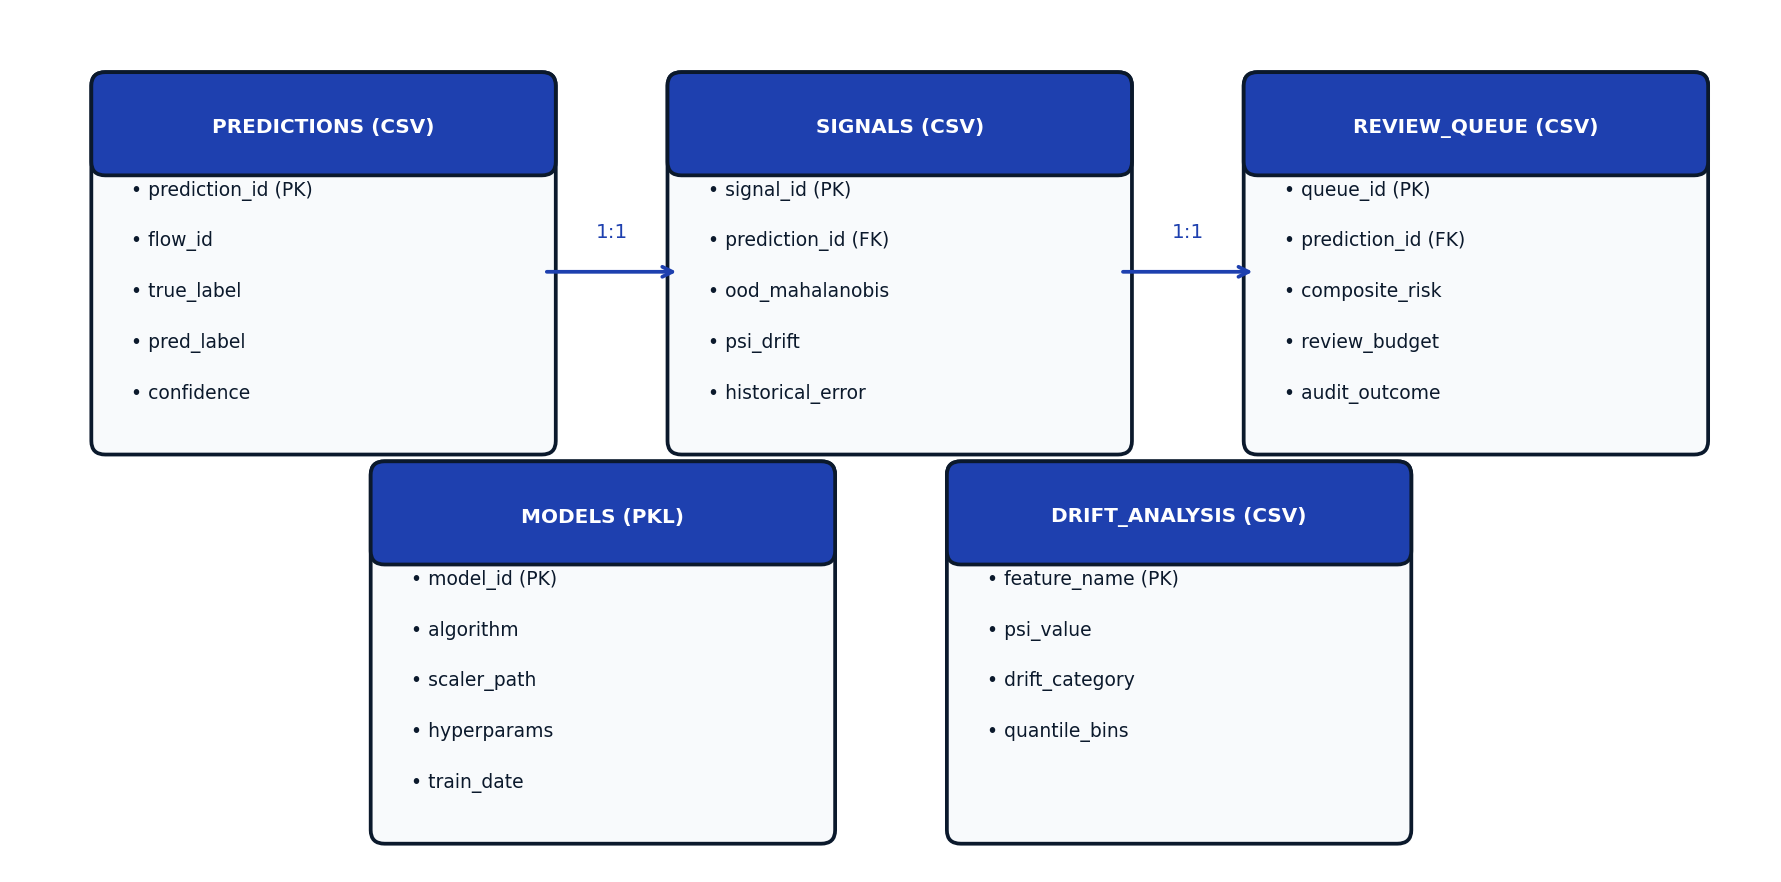
\includegraphics[width=0.85\textwidth]{figures/v2_er_diagram.png}
\caption{Figure 12.1: Conceptual Entity-Relationship Diagram for File-Based Storage Architecture.}
\end{figure}

\subsection{12.2 Conceptual Schema}

The logical schema maps to discrete CSV and binary artifacts residing in results/ and models/. Table 12.1 outlines the primary entities, attributes, data types, and integrity constraints for the file-based experiment architecture.

\begin{table}[H]
\centering
\small
\begin{tabular}{p{0.14\textwidth} p{0.16\textwidth} p{0.14\textwidth} p{0.18\textwidth} p{0.28\textwidth}}
\toprule
\textbf{Entity / File} & \textbf{Field Name} & \textbf{Data Type} & \textbf{Constraint} & \textbf{Description} \\
\midrule
PREDICTIONS & prediction\_id & Integer & PK, Unique & Deterministic zero-indexed inference ID. \\
PREDICTIONS & true\_label & Integer (0/1) & NOT NULL & Ground-truth class (0=Benign, 1=Attack). \\
PREDICTIONS & predicted\_label & Integer (0/1) & NOT NULL & Classifier decision at 0.5 threshold. \\
PREDICTIONS & confidence & Float [0,1] & NOT NULL & Max class posterior max(P, 1-P). \\
PREDICTIONS & actual\_error & Integer (0/1) & NOT NULL & Binary indicator (1 if y\_true != y\_pred). \\
SIGNALS & prediction\_id & Integer & FK, PK & Reference to PREDICTIONS table. \\
SIGNALS & confidence\_risk & Float [0,1] & NOT NULL & Normalized uncertainty (1 - confidence). \\
SIGNALS & ood\_percentile & Float [0,1] & NOT NULL & Empirical rank of Mahalanobis distance. \\
SIGNALS & drift\_risk & Float [0,1] & NOT NULL & Feature-weighted PSI vulnerability. \\
SIGNALS & historical\_risk & Float [0,1] & NOT NULL & Mistake density in feature decile bin. \\
REVIEW\_QUEUE & prediction\_id & Integer & FK, PK & Reference to PREDICTIONS table. \\
REVIEW\_QUEUE & composite\_risk & Float [0,1] & NOT NULL & Synthesized four-factor score. \\
REVIEW\_QUEUE & budget\_tier & Float & NOT NULL & Operational capacity (0.01, 0.02, 0.05, 0.10). \\
REVIEW\_QUEUE & audit\_confirmed & Integer (0/1) & NOT NULL & Simulated oracle verified error status. \\
DRIFT\_ANALYSIS & feature\_name & String & PK & Network flow attribute name. \\
DRIFT\_ANALYSIS & psi\_value & Float & NOT NULL & Population Stability Index metric. \\
DRIFT\_ANALYSIS & drift\_category & String & NOT NULL & Negligible (<0.1), Moderate, or Severe (>0.25). \\
\bottomrule
\end{tabular}
\caption{12.2 Conceptual Schema}
\end{table}

\subsection{12.3 NoSQL / Document Structure}

\textbf{Status:} Not Applicable. Network flow telemetry metrics are fundamentally tabular, numerical, and fixed-schema records. The operational pipeline relies entirely on structured tabular CSV matrices and NumPy arrays; no unstructured JSON document collections or NoSQL document stores are required.

\subsection{12.4 Dataset / Data Schema}

The project utilizes the BigFlow-NIDS benchmark (Uddin \& Arefin, Data in Brief 2026). BigFlow-NIDS is a large-scale derived network intrusion detection benchmark constructed from publicly available NetFlow datasets. Table 12.2 provides representative sample attributes from the 49 numerical flow features used for modeling.

\begin{table}[H]
\centering
\small
\begin{tabular}{p{0.1\textwidth} p{0.28\textwidth} p{0.38\textwidth} p{0.16\textwidth}}
\toprule
\textbf{Attribute Name} & \textbf{Data Type} & \textbf{Statistical Description} & \textbf{Example Value} \\
\midrule
flow\_duration & Float64 & Total duration of network flow in microseconds. & 104,230.0 \\
total\_fwd\_packets & Int64 & Total packets transmitted in forward direction. & 12 \\
total\_bwd\_packets & Int64 & Total packets transmitted in backward direction. & 8 \\
total\_fwd\_bytes & Float64 & Total bytes transmitted in forward direction. & 1,440.0 \\
total\_bwd\_bytes & Float64 & Total bytes transmitted in backward direction. & 4,820.0 \\
fwd\_packet\_length\_max & Float64 & Maximum length of forward packet in bytes. & 1,460.0 \\
flow\_iat\_mean & Float64 & Mean inter-arrival time between packets (microseconds). & 5,211.5 \\
flow\_packets\_per\_sec & Float64 & Flow throughput in packets per second. & 191.88 \\
fwd\_header\_length & Int64 & Total header bytes in forward direction. & 240 \\
init\_win\_bytes\_forward & Int64 & TCP initial window size in forward direction. & 65,535 \\
label & Int64 (Target) & Binary target class (0 = Benign flow, 1 = Attack flow). & 0 \\
\bottomrule
\end{tabular}
\caption{12.4 Dataset / Data Schema}
\end{table}

